\documentclass[aspectratio=169,10pt]{beamer}
\usepackage[UTF8]{ctex}

\usetheme{Madrid}
\usecolortheme{default}
\setbeamertemplate{navigation symbols}{}
\setbeamertemplate{footline}[frame number]

\usepackage{amsmath,amssymb,booktabs,mathtools,array}
\usepackage{graphicx}
\usepackage{hyperref}
\usepackage{tikz}
\usetikzlibrary{arrows.meta,positioning,fit}
\usepackage{ragged2e}

\definecolor{positive}{HTML}{0173B2}
\definecolor{negative}{HTML}{DE8F05}
\definecolor{emphasis}{HTML}{029E73}
\definecolor{neutral}{gray}{0.45}
\definecolor{buaaBlue}{HTML}{0B3A82}
\definecolor{softBlue}{HTML}{EAF2FF}
\definecolor{softOrange}{HTML}{FFF1E0}
\definecolor{softGreen}{HTML}{EAF7F1}
\newcommand{\pos}[1]{\textcolor{positive}{#1}}
\newcommand{\con}[1]{\textcolor{negative}{#1}}
\newcommand{\HL}[1]{\textcolor{emphasis}{#1}}
\newcommand{\RAG}{\text{RAG}}
\newcommand{\USTG}{\text{USTG}}
\newcommand{\TCAE}{\text{TCAE}}

\title{HomeAgent 项目介绍与本周设计汇报}
\subtitle{TCA 到 TCAE、RAG 与 USTG}
\author{汇报主题：理论推导与项目设计}
\institute{BUAA}
\date{2026-06-01}

\begin{document}

\begin{frame}
  \titlepage
\end{frame}

\begin{frame}{本周工作定位与汇报主线}
\begin{columns}[T]
  \column{0.52\textwidth}
  \textbf{本周重点：}
  \begin{itemize}
    \item \textbf{理论推导}：补全 \TCAE 建模、规则关联图、非预期状态转换图定义
    \item \textbf{项目设计}：把 Home Assistant 自动化文件转成可分析的图结构
    \item \textbf{目标聚焦}：不是传统 \textit{conflict}，而是\HL{由规则关联路径诱导出的非预期状态转换}
  \end{itemize}

  \vspace{4pt}
  \textbf{本次汇报回答 3 个问题：}
  \begin{enumerate}
    \item TCA 如何增加为 \TCAE
    \item \TCAE 与自动化规则文件如何生成 \RAG
    \item \RAG 如何结合常态配置剪枝生成 \USTG
  \end{enumerate}

  \column{0.44\textwidth}
  \begin{center}
  \begin{tikzpicture}[
    box/.style={draw, rounded corners, fill=softBlue, minimum width=2.45cm, minimum height=0.75cm, align=center, font=\small},
    arr/.style={-{Stealth}, thick, color=buaaBlue}
  ]
    \node[box] (yaml) {automations.yaml};
    \node[box, below=0.58cm of yaml] (tcae) {\TCAE 模型};
    \node[box, below=0.58cm of tcae] (rag) {规则关联图 \RAG};
    \node[box, below=0.58cm of rag] (norm) {实体常态配置};
    \node[box, below=0.58cm of norm] (ustg) {非预期状态转换图 \USTG};
    \draw[arr] (yaml) -- (tcae);
    \draw[arr] (tcae) -- (rag);
    \draw[arr] (rag) -- (norm);
    \draw[arr] (norm) -- (ustg);
  \end{tikzpicture}
  \end{center}
\end{columns}
\end{frame}

\begin{frame}{为什么要从 TCA 扩展到 \TCAE}
\begin{columns}[T]
  \column{0.48\textwidth}
  \textbf{传统 TCA：}
  \[
    r = \langle T_r, C_r, A_r \rangle
  \]
  \begin{itemize}
    \item 能表达\textbf{何时触发、何时允许、执行什么}
    \item 但缺少\con{环境依赖与环境传播}信息
    \item 因而难以描述：
      \begin{itemize}
        \item 数值型环境触发/条件
        \item 动作对温度、湿度、光照、水流等的影响
        \item 规则经由环境形成的间接关联路径
      \end{itemize}
  \end{itemize}

  \column{0.48\textwidth}
  \textbf{扩展后的 \TCAE：}
  \[
    r = \langle T_r, C_r, A_r, (E_r^T,E_r^C,E_r^A)\rangle
  \]
  \begin{itemize}
    \item $E_r^T$：Trigger 的环境引用集
    \item $E_r^C$：Condition 的环境引用集
    \item $E_r^A$：Action 的环境效应集
  \end{itemize}

  \vspace{4pt}
  \textbf{核心收益：}
  \begin{itemize}
    \item \pos{把环境参数显式纳入规则模型}
    \item \pos{允许构建组件级关联图而非只停留在规则级}
    \item \pos{为后续 \RAG 剪枝和 \USTG 生成提供依据}
  \end{itemize}
\end{columns}
\end{frame}

\begin{frame}{TCA 到 \TCAE：增加的不是 1 个字段，而是 3 类环境语义}
\begin{center}
\scriptsize
\begin{tabular}{>{\RaggedRight\arraybackslash}p{0.16\textwidth} >{\RaggedRight\arraybackslash}p{0.21\textwidth} >{\RaggedRight\arraybackslash}p{0.24\textwidth} >{\RaggedRight\arraybackslash}p{0.24\textwidth}}
\toprule
组件 & 形式 & 语义 & 项目中的典型例子 \\
\midrule
$E_r^T$ & $\rho=(z,c,\bowtie,\theta)$ & 触发器依赖区域-通道阈值变化 & 温度上穿 30 触发开窗 \\
$E_r^C$ & $\rho=(z,c,\bowtie,\theta)$ & 条件依赖当前环境阈值是否满足 & 光照 $<50$ 才允许开灯 \\
$E_r^A$ & $\eta=(z_s,\mathcal{R},c,s,\mu,\lambda,d)$ & 动作对环境参数的方向、范围与持续影响 & 加热器升温；阀门关闭使水流下降 \\
\bottomrule
\end{tabular}
\end{center}

\vspace{4pt}
\textbf{形式化增量：}
\[
\operatorname{RefEnv}(T_r),\; \operatorname{RefEnv}(C_r),\; \Gamma(A_r)
\]
\begin{itemize}
  \item 前两者提取 Trigger/Condition 中的\textbf{环境引用}
  \item 最后一项把执行器动作映射成\textbf{环境效应}
  \item 因而规则不仅有离散实体后态，还能表达环境传播后果
\end{itemize}
\end{frame}

\begin{frame}{从自动化规则文件生成 \TCAE：项目里的实际链路}
\begin{columns}[T]
  \column{0.53\textwidth}
  \begin{center}
  \begin{tikzpicture}[
    box/.style={draw, rounded corners, minimum width=2.45cm, minimum height=0.72cm, align=center, font=\small},
    bluebox/.style={box, fill=softBlue},
    greenbox/.style={box, fill=softGreen},
    orangebox/.style={box, fill=softOrange},
    arr/.style={-{Stealth}, thick}
  ]
    \node[bluebox] (a0) {automations.yaml};
    \node[greenbox, below=0.48cm of a0] (a1) {脚本1：实体提取 + channel 绑定};
    \node[greenbox, below=0.48cm of a1] (a2) {脚本2：zone 绑定 + \TCAE 构建};
    \node[orangebox, below left=0.48cm and -0.15cm of a2] (o1) {devices.json / channels.json};
    \node[orangebox, below right=0.48cm and -0.15cm of a2] (o2) {zones.json / tcae.json};
    \draw[arr] (a0) -- (a1);
    \draw[arr] (a1) -- (a2);
    \draw[arr] (a1) -- (o1);
    \draw[arr] (a2) -- (o2);
  \end{tikzpicture}
  \end{center}

  \column{0.43\textwidth}
  \textbf{当前工程产物（已生成）：}
  \begin{itemize}
    \item 规则数：\textbf{17}
    \item 环境触发引用数：\textbf{6}
    \item 环境条件引用数：\textbf{5}
    \item 动作环境效应数：\textbf{38}
  \end{itemize}

  \vspace{4pt}
  \textbf{关键设计点：}
  \begin{itemize}
    \item channel 绑定决定\textbf{实体对应哪些物理通道}
    \item zone 绑定决定\textbf{环境效应从何处产生、向何处传播}
    \item 二者缺一不可，否则难以落到环境图节点
  \end{itemize}
\end{columns}
\end{frame}

\begin{frame}{\TCAE 如何生成规则关联图 \RAG}
\begin{columns}[T]
  \column{0.50\textwidth}
  \textbf{节点拆分：}
  \[
    V = V^T \cup V^C \cup V^A \cup V^E
  \]
  \begin{itemize}
    \item 触发器节点 $v_r^T$
    \item 条件节点 $v_r^C$
    \item 动作节点 $v_r^A$
    \item 环境参数节点 $v_{z,c}^E$
  \end{itemize}

  \vspace{4pt}
  \textbf{规则内部边：}
  \[
    T_r \rightarrow C_r \rightarrow A_r \quad \text{或} \quad T_r \rightarrow A_r
  \]

  \column{0.47\textwidth}
  \textbf{规则关联边：}
  \begin{itemize}
    \item \textbf{直接边}：$A \rightarrow T,\; A \rightarrow C,\; A \rightarrow A$
    \item \textbf{环境边}：$A \rightarrow E,\; E \rightarrow T,\; E \rightarrow C,\; E \rightarrow A$
  \end{itemize}

  \vspace{4pt}
  \begin{center}
  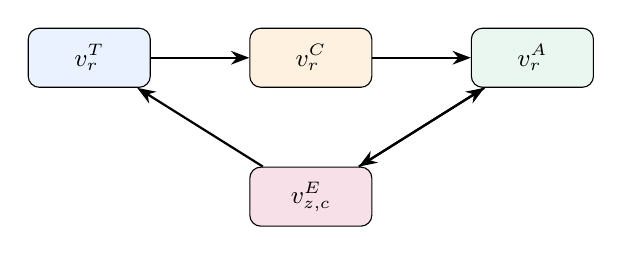
\begin{tikzpicture}[
    n/.style={draw, rounded corners, minimum width=1.55cm, minimum height=0.75cm, font=\small, align=center},
    arr/.style={-{Stealth}, thick}
  ]
    \node[n, fill=softBlue] (T) {$v_r^T$};
    \node[n, fill=softOrange, right=1.25cm of T] (C) {$v_r^C$};
    \node[n, fill=softGreen, right=1.25cm of C] (A) {$v_r^A$};
    \node[n, fill=purple!12, below=1.0cm of C] (E) {$v_{z,c}^E$};
    \draw[arr] (T) -- (C);
    \draw[arr] (C) -- (A);
    \draw[arr] (A) -- (E);
    \draw[arr] (E) -- (T);
    \draw[arr] (E) -- (A);
  \end{tikzpicture}
  \end{center}
\end{columns}
\end{frame}

\begin{frame}{当前项目生成的 \RAG 规模与边类型}
\begin{columns}[T]
  \column{0.52\textwidth}
  \begin{center}
  \small
  \begin{tabular}{lrr}
  \toprule
  指标 & 数值 & 说明 \\
  \midrule
  节点总数 & 48 & 17T + 9C + 17A + 5E \\
  边总数 & 95 & 26 内部边 + 69 关联边 \\
  规则数 & 17 & 当前 HomeAgent 示例工程 \\
  \bottomrule
  \end{tabular}
  \end{center}

  \vspace{4pt}
  \begin{center}
  \small
  \begin{tabular}{lr}
  \toprule
  边类型 & 当前数量 \\
  \midrule
  flow & 26 \\
  env-association $(A\rightarrow E)$ & 21 \\
  indirect-action $(E\rightarrow A)$ & 21 \\
  direct-action $(A\rightarrow A)$ & 12 \\
  env-trigger $(E\rightarrow T)$ & 6 \\
  indirect-condition-disable $(E\rightarrow C)$ & 5 \\
  direct-trigger $(A\rightarrow T)$ & 2 \\
  direct-condition-allow $(A\rightarrow C)$ & 2 \\
  \bottomrule
  \end{tabular}
  \end{center}

  \column{0.44\textwidth}
  \textbf{解读：}
  \begin{itemize}
    \item 当前图里\HL{环境相关边占主导}，说明环境传播是主要关联来源
    \item $A\rightarrow E$ 与 $E\rightarrow A$ 同时存在，允许形成\textbf{经由环境的动作-动作关联路径}
    \item 当前实例中未出现 direct-condition-disable 与 indirect-condition-allow，但\textbf{理论定义已支持}
  \end{itemize}
\end{columns}
\end{frame}

\begin{frame}{规则关联图示例（按用户提供图片直接使用）}
\begin{columns}[T]
  \column{0.70\textwidth}
  \begin{center}
    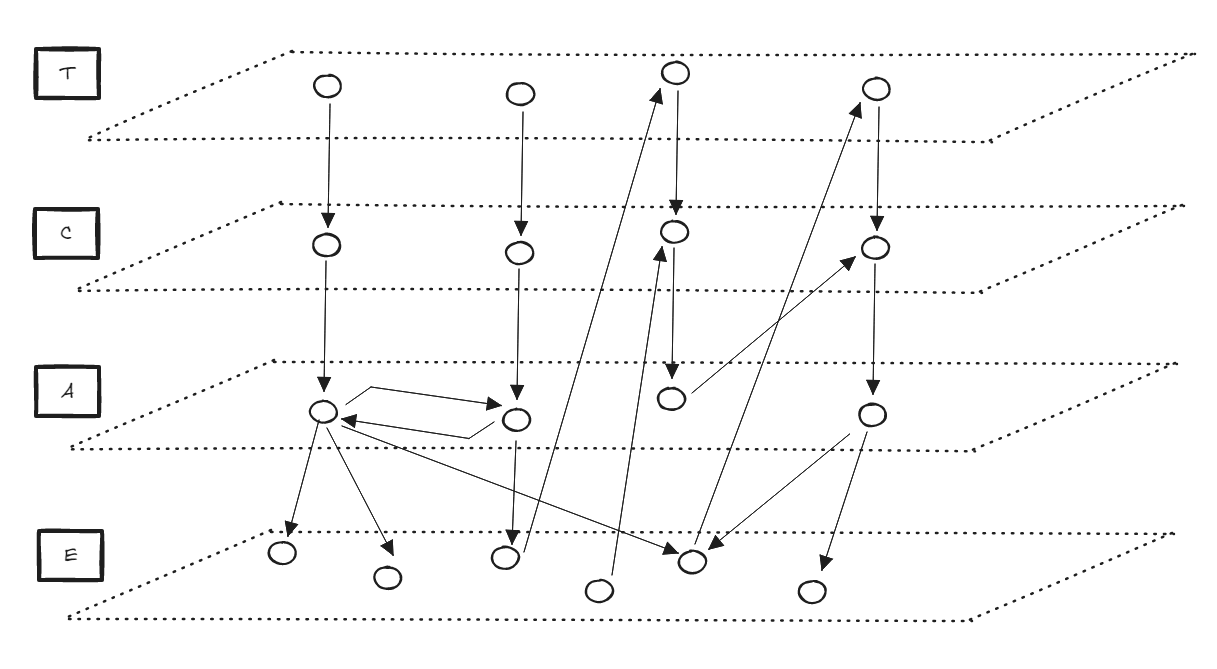
\includegraphics[width=\textwidth]{assets/example_RAG.png}
  \end{center}

  \column{0.27\textwidth}
  \textbf{读图方式：}
  \begin{itemize}
    \item 上到下分别为：\textbf{T / C / A / E}
    \item 竖向边体现\textbf{规则内部流程}
    \item 斜向或跨层边体现\textbf{规则关联或环境中介}
    \item 本页仅展示\textbf{结构样式}，不改动画线方向与数量
  \end{itemize}

  \vspace{4pt}
  \textcolor{neutral}{说明：该图按用户给定文件直接拷贝到 beamer 资产目录中使用。}
\end{columns}
\end{frame}

\begin{frame}{从 \RAG 到 \USTG：先引入实体常态配置}
\begin{columns}[T]
  \column{0.53\textwidth}
  \textbf{静态阶段的判定核心：}
  \[
    \operatorname{Abn}_{\mathcal N}(v_r^A)
    \Longleftrightarrow
    \exists (e,v')\in \operatorname{Post}(v_r^A),\; N_e(v')=0
  \]
  \begin{itemize}
    \item 只要动作后态 $v'$ 落在实体非常态集合，就把该动作节点标为\HL{异常终点候选}
    \item 这是一种\textbf{弱非预期后态}判定：静态阶段只看目标后态，不依赖运行时前态
  \end{itemize}

  \column{0.44\textwidth}
  \begin{center}
  \small
  \begin{tabular}{lll}
  \toprule
  实体 & 常态值 & 等级 \\
  \midrule
  中央水阀 & on & critical \\
  消防喷淋头 & off & critical \\
  智能门锁 & off & high \\
  卧室窗户 & off & high \\
  温室窗户 & off & high \\
  \bottomrule
  \end{tabular}
  \end{center}

  \vspace{4pt}
  \textbf{由常态得到的 5 个异常终点：}
  \begin{itemize}
    \item R10：水阀 \texttt{off}
    \item R11：喷淋头 \texttt{on}
    \item R14：卧室窗户 \texttt{on}
    \item R17：温室窗户 \texttt{on}
    \item R2：门锁 \texttt{on}
  \end{itemize}
\end{columns}
\end{frame}

\begin{frame}{\RAG 如何结合常态配置剪枝生成 \USTG}
\begin{columns}[T]
  \column{0.56\textwidth}
  \textbf{剪枝通过保留“能到达异常终点的关联路径”实现：}
  \[
    \mathcal P_U = \{p \mid \operatorname{UOutcome}_{\mathcal N}(p)\}
  \]
  \[
    V_U = \{v\in V \mid \exists p\in\mathcal P_U, v\in p\},\; E_U = \{e\in E \mid \exists p\in\mathcal P_U, e\in p\}
  \]

  \textbf{算法过程：}
  \begin{itemize}
    \item 先从 \TCAE 读取每个动作节点的后态集合
    \item 用 \texttt{normal\_config.json} 标出\textbf{5 个异常动作节点}
    \item 以异常动作节点为终点，在 \RAG 上做\textbf{有界反向 DFS}
    \item 仅保留包含至少一条关联边的路径对应子图，得到 \USTG
  \end{itemize}

  \column{0.40\textwidth}
  \begin{center}
  \small
  \begin{tabular}{lrr}
  \toprule
  图/指标 & 节点 & 边 \\
  \midrule
  原始 \RAG & 48 & 95 \\
  剪枝后 \USTG & 41 & 65 \\
  \bottomrule
  \end{tabular}
  \end{center}

  \vspace{4pt}
  \begin{itemize}
    \item 异常动作节点：\textbf{5}
    \item 非预期关联路径：\textbf{294}
    \item 路径极性：95 条正极性，199 条负极性
  \end{itemize}
\end{columns}
\end{frame}

\begin{frame}{当前 \USTG 的 5 个终止异常动作}
\begin{center}
\scriptsize
\begin{tabular}{>{\RaggedRight\arraybackslash}p{0.16\textwidth} >{\RaggedRight\arraybackslash}p{0.22\textwidth} c c c}
\toprule
终止规则 & 异常实体 & 常态值 & 异常后态 & 路径数 \\
\midrule
R10 Water Shutoff & central water valve & on & off & 4 \\
R11 Fire Suppression & fire sprinkler & off & on & 4 \\
R14 Bedroom Window & bedroom window & off & on & 84 \\
R17 Greenhouse Window & greenhouse window & off & on & 84 \\
R2 Door Unlock & smart door lock & off & on & 118 \\
\bottomrule
\end{tabular}
\end{center}

\vspace{4pt}
\textbf{观察：}
\begin{itemize}
  \item 门锁与窗户属于\HL{安全敏感实体}，因此 on/open 会被保留为异常终点
  \item 水阀与喷淋头说明模型不仅关注门窗，也覆盖水流与消防链路
  \item R2 路径数最多，说明“离家关灯”与“重新开灯并解锁”之间存在更复杂传播
\end{itemize}
\end{frame}

\begin{frame}{本周产出总结与后续工作}
\begin{columns}[T]
  \column{0.50\textwidth}
  \textbf{本周已完成：}
  \begin{itemize}
    \item \textbf{理论定义完备}：实体、环境、\TCAE、\RAG、\USTG
    \item \textbf{工程链路打通}：
      \begin{itemize}
        \item 脚本1：实体提取与 channel 绑定
        \item 脚本2：zone 绑定与 \TCAE 构建
        \item 脚本3：\RAG 生成
        \item 脚本4：常态配置生成
        \item 脚本5：\USTG 剪枝生成
      \end{itemize}
    \item \textbf{当前状态}：已经可以从自动化文件走到非预期状态转换图
  \end{itemize}

  \column{0.46\textwidth}
  \textbf{下一步重点：}
  \begin{itemize}
    \item 图游走与运行时验证策略
    \item 规则关联边定义与实例库完善
    \item 冲突/非预期案例设计与实验评价
    \item 处理规则生成与人工可审查输出
  \end{itemize}

  \vspace{4pt}
  \textbf{一句话总结：}
  \begin{itemize}
    \item \HL{本周的核心成果是把“自动化规则”提升为“可做环境关联与异常剪枝的图模型”。}
  \end{itemize}
\end{columns}
\end{frame}

\begin{frame}{References}
\small
\begin{thebibliography}{9}
  \bibitem{homeagent-readme}
  HomeAgent Project.
  \newblock \textit{README.md: theoretical definitions and project workflow}, 2026.

  \bibitem{homeagent-step2}
  HomeAgent Project.
  \newblock \texttt{src/2\_bind\_zones\_and\_build\_tcae.py}, 2026.

  \bibitem{homeagent-step3}
  HomeAgent Project.
  \newblock \texttt{src/3\_build\_rule\_association\_graph.py}, 2026.

  \bibitem{homeagent-step5}
  HomeAgent Project.
  \newblock \texttt{src/5\_build\_unexpected\_state\_transition\_graph.py}, 2026.

  \bibitem{ha-doc}
  Home Assistant.
  \newblock \textit{Automation documentation and YAML rule model}, accessed 2026.
\end{thebibliography}
\end{frame}

\begin{frame}{Thank You}
\begin{center}
  {\LARGE 谢谢！}\\[8pt]
  {\large Q\&A}
\end{center}
\end{frame}

\appendix

\begin{frame}{Backup Slides}
\end{frame}

\begin{frame}{Backup 1：边类型与当前实例计数}
\begin{center}
\small
\begin{tabular}{lrr}
\toprule
边类型 & 方向 & 数量 \\
\midrule
flow & $T\rightarrow C\rightarrow A$ 或 $T\rightarrow A$ & 26 \\
direct-trigger & $A\rightarrow T$ & 2 \\
direct-condition-allow & $A\rightarrow C$ & 2 \\
direct-action & $A\rightarrow A$ & 12 \\
env-association & $A\rightarrow E$ & 21 \\
env-trigger & $E\rightarrow T$ & 6 \\
indirect-action & $E\rightarrow A$ & 21 \\
indirect-condition-disable & $E\rightarrow C$ & 5 \\
\bottomrule
\end{tabular}
\end{center}

\vspace{6pt}
\textbf{注意：}
\begin{itemize}
  \item 当前实例计数来自 \texttt{rule\_association\_graph.json} 实际汇总
  \item 理论上还支持 direct-condition-disable 与 indirect-condition-allow；本实例暂未出现
\end{itemize}
\end{frame}

\begin{frame}{Backup 2：两条来自当前 \USTG 的真实路径样例}
\small
\textbf{样例 A：R15 $\rightarrow$ R2（直接触发门锁异常）}
\[
\texttt{R15::A} \rightarrow \texttt{R2::T} \rightarrow \texttt{R2::A}
\]
\begin{itemize}
  \item 边类型序列：\texttt{direct-trigger}, \texttt{flow}
  \item 终点异常：门锁后态 \texttt{on}，而常态为 \texttt{off}
  \item 路径极性：$+1$
\end{itemize}

\vspace{6pt}
\textbf{样例 B：R11 $\rightarrow E_{water\_flow} \rightarrow$ R10（经由环境影响水阀链路）}
\[
\texttt{R11::A} \rightarrow \texttt{env::home::water\_flow} \rightarrow \texttt{R10::A}
\]
\begin{itemize}
  \item 边类型序列：\texttt{env-association}, \texttt{indirect-action}
  \item 终点异常：中央水阀后态 \texttt{off}，而常态为 \texttt{on}
  \item 路径极性：$-1$
\end{itemize}
\end{frame}

\begin{frame}{Backup 3：工程脚本与输出文件对应关系}
\begin{center}
\tiny
\begin{tabular}{>{\RaggedRight\arraybackslash}p{0.31\textwidth} >{\RaggedRight\arraybackslash}p{0.57\textwidth}}
\toprule
脚本 & 主要输出 \\
\midrule
\texttt{1\_extract\_devices\_and\_bind\_channels.py} & \texttt{devices.json}, \texttt{channels.json} \\
\texttt{2\_bind\_zones\_and\_build\_tcae.py} & \texttt{zones.json}, \texttt{tcae.json} \\
\texttt{3\_build\_rule\_association\_graph.py} & \texttt{rule\_association\_graph.json} \\
\texttt{4\_generate\_normal\_config.py} & \texttt{normal\_config.json} \\
\texttt{5\_build\_unexpected\_state\_transition\_graph.py} & \texttt{unexpected\_state\_transition\_graph.json} \\
\texttt{6\_generate\_resolution\_rules.py} & \texttt{resolution\_rules.json} \\
\bottomrule
\end{tabular}
\end{center}

\vspace{6pt}
\textbf{因此本项目的最小闭环是：}
\[
\texttt{automations.yaml} \Rightarrow \TCAE \Rightarrow \RAG \Rightarrow \USTG
\]
\end{frame}

\end{document}
